\section{Calculo lambda}
\begin{itemize}
\item Surge en la década del 30, estaban interesados en saber cuando una función es computable.
\item Todo es una función en calculo $\lambda$ , incluso un numero.
\end{itemize}

\subsection*{Ejemplo: Función sucesor}
\begin{center}
    $succ(x) = x + 1$
\end{center}


\begin{itemize}
\item succ es el nombre de la función
\item x es el parámetro (formal) en la definición de la función
\item x+1 es el cuerpo de la función
\end{itemize}


Si llamo a succ con el numero 4, 4 seria el argumento (efectivo). Argumento se dice en la invocación

Las funciones pueden entonces no tener un nombre, se indican con una flecha

\begin{center}
$x \rightarrow x + 1$
\end{center}

El calculo lambda no tiene entrada salida de forma directa.

Los programas en programación funcional son muchas funciones. En calculo lambda se llaman expresiones.

\subsection*{Programas como expresiones}

Un programa funcional consiste en una expresión E que representa tanto al algoritmo como los datos de entrada. Para ejecutarla se le aplican a E reglas de conversión.

\begin{center}
$E[P] \rightarrow E[P']$
\end{center}

\begin{itemize}
\item La reducción consiste en remplazar una parte de P de E por otra expresión P'. $P \rightarrow P'$ debe estar de acuerdo con las reglas.
\item La reducción se repite hasta que la expresión resultante no tenga mas partes que puedan convertirse. Se llama forma normal E* de la expresión E consiste en la salida del programa funcional dado.
\item Llamamos combinadores a funciones que combinan algunas reglas de conversión.
\item Los sistemas de reducción satisfacen la propiedad de Church-Rosser. Esto establece que la forma normal obtenida es independiente del orden de reducción de los subterminos.
\item Tenemos que tener alguna forma de manejar la situación si alguna operación no se puede realizar
\end{itemize}


\subsection*{Sintaxis del calculo lambda}

La sintaxis de una expresión lambda se puede expresar como BNF (Backus-Naur-Form)


\begin{equation*} \label{eq1}
\begin{split}
<expresion \lambda> ::= & <variable> |\\
& (\lambda <variable>.<expresion \lambda>) |\\
& (<expresion \lambda><expresion \lambda>)
\end{split}
\end{equation*}


Es una de las siguientes 3 opciones
\begin{itemize}
\item Una variable (primer termino)
\item Una abstracción: con una variable (o parámetro) y un cuerpo que también es una expresión lambda (segundo termino)
\item Una aplicación: que tiene un operador (función) y un operando (argumento) que son también ambos expresiones lambda. Se diferencia de antes, en que no va entre paréntesis el argumento, todo va entre paréntesis (tercer termino)
\end{itemize}


La posición determina que es, a la izquierda el operador (la función), a la derecha el operando (los argumentos)
El BNF aporta los <>, ::= , |
Entre paréntesis se ponen cosas evaluables.
En calculo lambda solo se puede pasar un solo argumento, para pasar varios, se van anidando de a pares.

\subsubsection*{Convenciones}
Aplicando las siguientes reglas se obtiene una expresión equivalente a la original.

\begin{center}
\begin{math}
(((\lambda x.(\lambda y.(y x))) a) b)
\end{math}  
\end{center}



\begin{enumerate}
    
\item Se omiten paréntesis externos.

\begin{center}
\begin{math}
((\lambda x.(\lambda y.(y x))) a) b 
\end{math}  
\end{center}


\item Se asume que las aplicaciones se asocian a la izquierda.

\begin{center}
\begin{math}
(\lambda x.(\lambda y.(y x))) a b
\end{math}  
\end{center}

\item Se asume que el cuerpo de las abstracciones se extiende hasta que se cierra un paréntesis o se alcanza el final de la expresión.

\begin{center}
\begin{math}
(\lambda x.\lambda y.y x) a b
\end{math}  
\end{center}

\item Opcionalmente se pueden contraer múltiples abstracciones lambda (se pueden sacar los lambda intermedios)

\begin{center}
\begin{math}
(\lambda x y.y x) a b
\end{math}  
\end{center}

\end{enumerate}

Currificacion 'curryng': técnica para invocar una función con menos parámetros de los que esperaría


\subsection*{Variables libres y ligadas}
\begin{figure}[!htb]
    \centering
    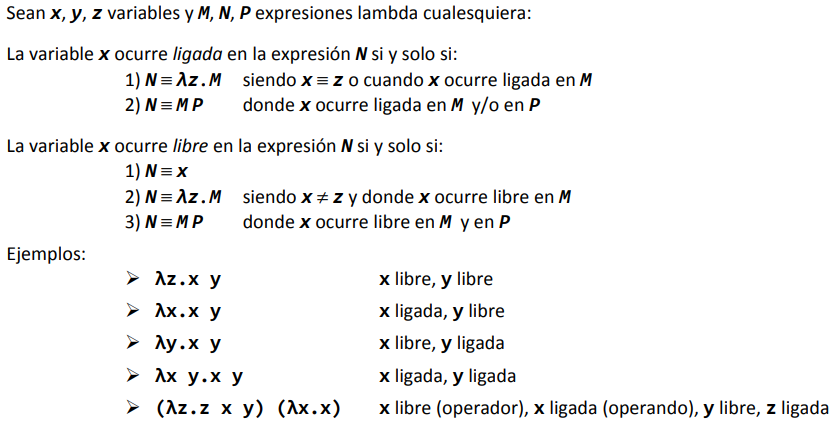
\includegraphics[width=\textwidth]{img/VariablesLigadas.PNG}
\end{figure}

La notación es que se le hacen arcos a los correspondientes parámetros. Se le puede poner arriba la inicial de que tipo es (en español es tienen ambas L, pero en ingles F(ree) y B(ound))

En las variables ligadas es en donde se hace el remplazo del argumento.

\newpage 

\subsection*{Reglas de conversión}
Son reglas que transforman una expresión en otra.

\subsubsection*{Alfa}
Es un renombre de la variable en una abstracción que tiene la forma $\lambda x.M$
Si la variable y no ocurre libre en M, es posible sustituir por y todas las ocurrencias libres de x en M.

\begin{center}
\begin{math}
\lambda x.M =_{\alpha} \lambda y.M[\,y/x]\,
\end{math}  
\end{center}

Esta regla solo se puede aplicar con las variables ligadas. 
La convención de Barendregt dice que no se recomienda que estén de ambos lados una variable con el mismo nombre (la x)

\begin{figure}[!htb]
    \centering
    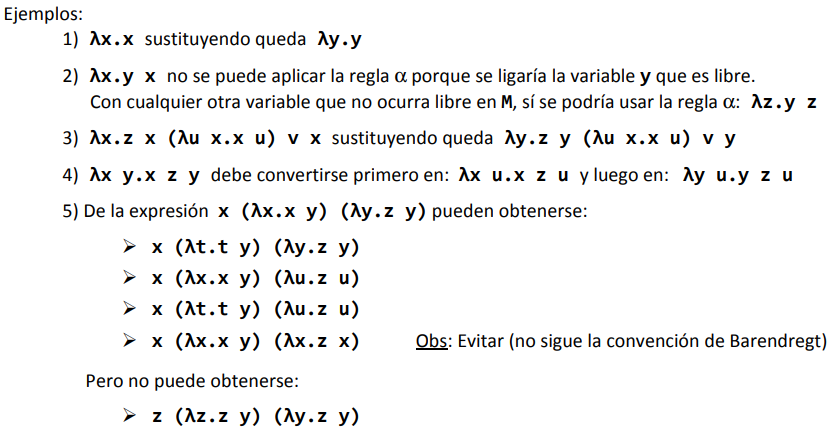
\includegraphics[width=\textwidth]{img/EjemplosConversionAlfa.PNG}
\end{figure}

\newpage 

\subsubsection*{Beta}
Se identifican $\beta-redex$ (expresión reducible $\beta$), que son una aplicación cuyo operador es una abstracción (tiene la forma $(\lambda x.M) N$). La regla beta la puedo usar solo para aplicaciones.

Ejemplos de $\beta$-redex.
\begin{figure}[!htb]
    \centering
    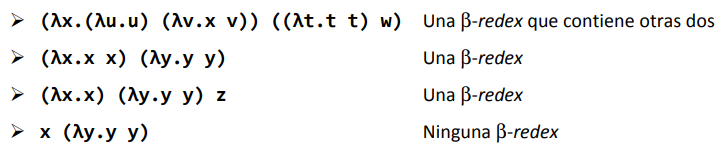
\includegraphics[width=\textwidth]{img/EjemplosBetaRedex.PNG}
\end{figure}

Una expresión lambda que no contiene ninguna $\beta$-redex está en forma normal. Mientras no se llegue a la forma normal, puede seguir aplicándose la regla de conversión Beta, que consiste en sustituir por N todas las ocurrencias libres de x en M. Es decir, la regla dice que hay que remplazar en el cuerpo, los parámetros por los argumentos.

\begin{center}
\begin{math}
(\lambda x.M) N =_{\beta} M[\,N/x]\,
\end{math}  
\end{center}

Aplicaciones:
\begin{figure}[!htb]
    \centering
    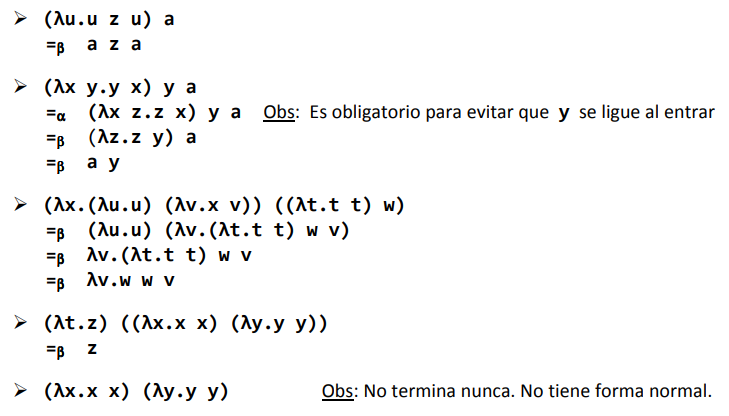
\includegraphics[width=\textwidth]{img/EjemplosAplicacionBeta.PNG}
\end{figure}

\newpage 
\subsubsection*{Eta}
Esta casi no se usa.

Consiste en realizar la reducción de una $\eta$-redex que es una abstracción con la forma '$\lambda$v.M v' en el cual 'v'\textbf{ no ocurre libre en M}. (Viendo solo M, independientemente del exterior)

\begin{center}
$\lambda v.M v =_{\eta} M$
\end{center}

\begin{figure}[!htb]
    \centering
    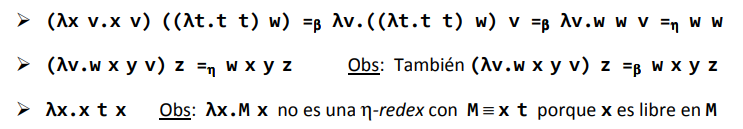
\includegraphics[width=0.8\textwidth]{img/EjemplosEta.PNG}
\end{figure}

\subsection*{Estrategias de reducción}

\subsubsection*{Call by name}
consiste en ir reduciendo siempre la $\beta$-redex \textbf{mas externa desde la izquierda} y que no este ubicada dentro de una abstracción lamba (cuerpo de una función), hasta llegar a una expresión en forma normal de cabecera (\textbf{head normal form}) Puede no coincidir con la forma normal. (Se termina cuando a la izquierda no tengo $\beta$-redex)

\begin{figure}[!htb]
    \centering
    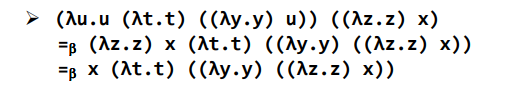
\includegraphics[width=0.7\textwidth]{img/CallByNameEjemplo.PNG}
\end{figure}


\subsubsection*{Orden normal}
Consiste en ir reduciendo siempre la $\beta$-redex mas externa desde la izquierda.

\begin{figure}[!htb]
    \centering
    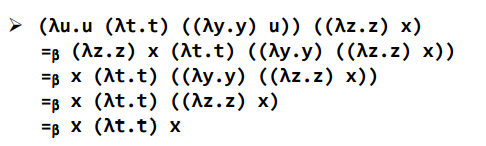
\includegraphics[width=0.7\textwidth]{img/OrdenNormalEj.PNG}
\end{figure}


\subsubsection*{Call by value}
Consiste en ir reduciendo siempre la $\beta$-redex mas interna desde la izquierda y que no este ubicada dentro de una abstracción lambda.

\begin{figure}[!htb]
    \centering
    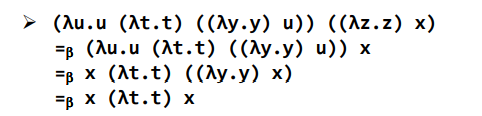
\includegraphics[width=0.7\textwidth]{img/CallByValueEj.PNG}
\end{figure}


\subsubsection*{Orden aplicativo}
Consiste en ir reduciendo siempre la $\beta$-redex mas interna desde la izquierda.

\begin{figure}[!htb]
    \centering
    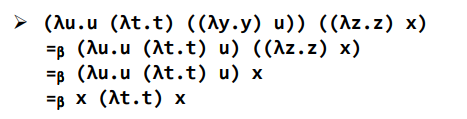
\includegraphics[width=0.7\textwidth]{img/OrdenAplicativoEj.PNG}
\end{figure}


\subsection*{Representación de valores de verdad, funciones lógicas}

\begin{itemize}
\item If = $\lambda$p . $\lambda$q.$\lambda$r. p q r
\item True = $\lambda$x. $\lambda$y.x
\item False = $\lambda$x. $\lambda$y.y
\item \textbf{If True b c} devuelve b
\item \textbf{If False b c} devuelve c
\item Not =  $\lambda$p.p False True =  $\lambda$p.p ($\lambda$x. $\lambda$y.y) ($\lambda$x. $\lambda$y.x)
\item And = $\lambda$p.$\lambda$q.p q False
\item Or = $\lambda$p.$\lambda$q. p True q
\item Xor = $\lambda$p.$\lambda$q.p (q False True) q
\end{itemize}

En base a la definición de funciones, y las reglas de reducción, se llega a formar un lenguaje de programación.

\subsection*{Representación de números, funciones numéricas y relacionales}
Se llaman numerales (representaciones de números)

\begin{itemize}
\item 0 = $\lambda$f.$\lambda$x.x
\item 1 = $\lambda$f.$\lambda$x.f x
\item 2 = $\lambda$f.$\lambda$x.f (f x)
\item ...
\end{itemize}
Si contamos la cantidad de f en el cuerpo sabemos a que numero estamos haciendo referencia.


\begin{itemize}
\item Succ = $\lambda$n.$\lambda$f.$\lambda$x.f (n f x)
\item Pred = $\lambda$n.$\lambda$f.$\lambda$x.n ($\lambda$g.$\lambda$h.h (g f)) ($\lambda$u.x) ($\lambda$u.u)
\item Add = $\lambda$m.$\lambda$n.$\lambda$f.$\lambda$x.m f (n f x)
\item Sub = $\lambda$m.$\lambda$n.n Pred m
\item Mul = $\lambda$m.$\lambda$n.$\lambda$f.$\lambda$x.m (n f) x
\item Pow = $\lambda$m.$\lambda$n.$\lambda$f.$\lambda$x.n m f x 
\item Fibo = $\lambda$n.n ($\lambda$f.$\lambda$a.$\lambda$b.f b (Add a b)) ($\lambda$x.$\lambda$y.x) ($\lambda$f.$\lambda$x.x) ($\lambda$f.$\lambda$x.f x) 
\item IsZero = $\lambda$n.n ($\lambda$z.($\lambda$x.$\lambda$y.y)) ($\lambda$x.$\lambda$y.x)
\end{itemize}

Basándonos en el IsZero, podemos encontrar la forma de representar las otras Gte, Lte, Lt, Gt, Eq

\begin{itemize}
\item Lte = $\lambda$x.$\lambda$y.Iszero (Sub x y)
\item Gte = $\lambda$x.$\lambda$y.Lte y x
\item Lt = $\lambda$x.$\lambda$y.Not (Gte x y) 
\item Gt = $\lambda$x.$\lambda$y.Not (Lte x y) 
\item Eq = $\lambda$x.$\lambda$y.And (Lte x y) (Gte x y)
\item Ne = $\lambda$x.$\lambda$y.Not (Eq x y)
\end{itemize}

\subsection*{Combinadores}
\begin{itemize}
\item No tienen variables libres, los usamos para representar ciclos. (El Y y el $\omega$?)
\item SKI es un tipo de logica combinatoria. Todo calculo lambda puede reformularse a SKI. 
\item SKI tiene solo una operación básica, la aplicación.
\item Fusión: S = $\lambda$x.$\lambda$y.$\lambda$z.x z (y z)
\item Constancia: K = $\lambda$x.$\lambda$y.x 
\item Identidad: K = $\lambda$x.$\lambda$y.x 
\end{itemize}


\subsection*{Pares y listas}

\begin{itemize}
\item Se tienen estructuras y tipos de datos, pares ordenados y listas en calculo lambda.
\item Un par ordenado esta compuesto por dos elementos, el primero y el segundo.
\end{itemize}

\begin{center}
(a.b) = $\lambda$s.s a b
\end{center}


\begin{itemize}
\item (a.b) es como se veria de forma externa.
\item La función Pair se usa para construir pares ordenados.
\end{itemize}


\begin{center}
Pair = $\lambda$x.$\lambda$y.$\lambda$s.s x y
\end{center}

Podemos definir la función First y Second.

\begin{itemize}
\item First = $\lambda$p.p True 
\item Second = $\lambda$p.p False 
\end{itemize}

La lista vacía se define de la forma:

\begin{itemize}
\item Nil = Pair True True o Nil = $\lambda$z.z
\end{itemize}

Construimos nodos con CONS. 
(CONS a (CONS b (CONS c Nil)))

Para verificar si la lista esta vacía, me fijo con Null = First. 

Para saber donde esta el final, recorro la lista buscando donde esta el Nil. (Tail)

Al comienzo, si no esta vacia y hacemos First, devuelve False. (se forma en la estructura)

